It is provided now a comparison among different regulators developed throughout the project work. \\ Since the pole placement approach was mainly used to test both the state reconstructors and the state space control scheme, this technique will not be introduced in the juxtaposition, also due to the presence of its optimal formulation, $LQG$.
The comparison will be so made among the proportional controller (exploiting the cascade strategy), $LQG$ and finally $H_{\infty}$.
\begin{figure*}[h]
	\centering
	\begin{subfigure}{0.45\columnwidth}
		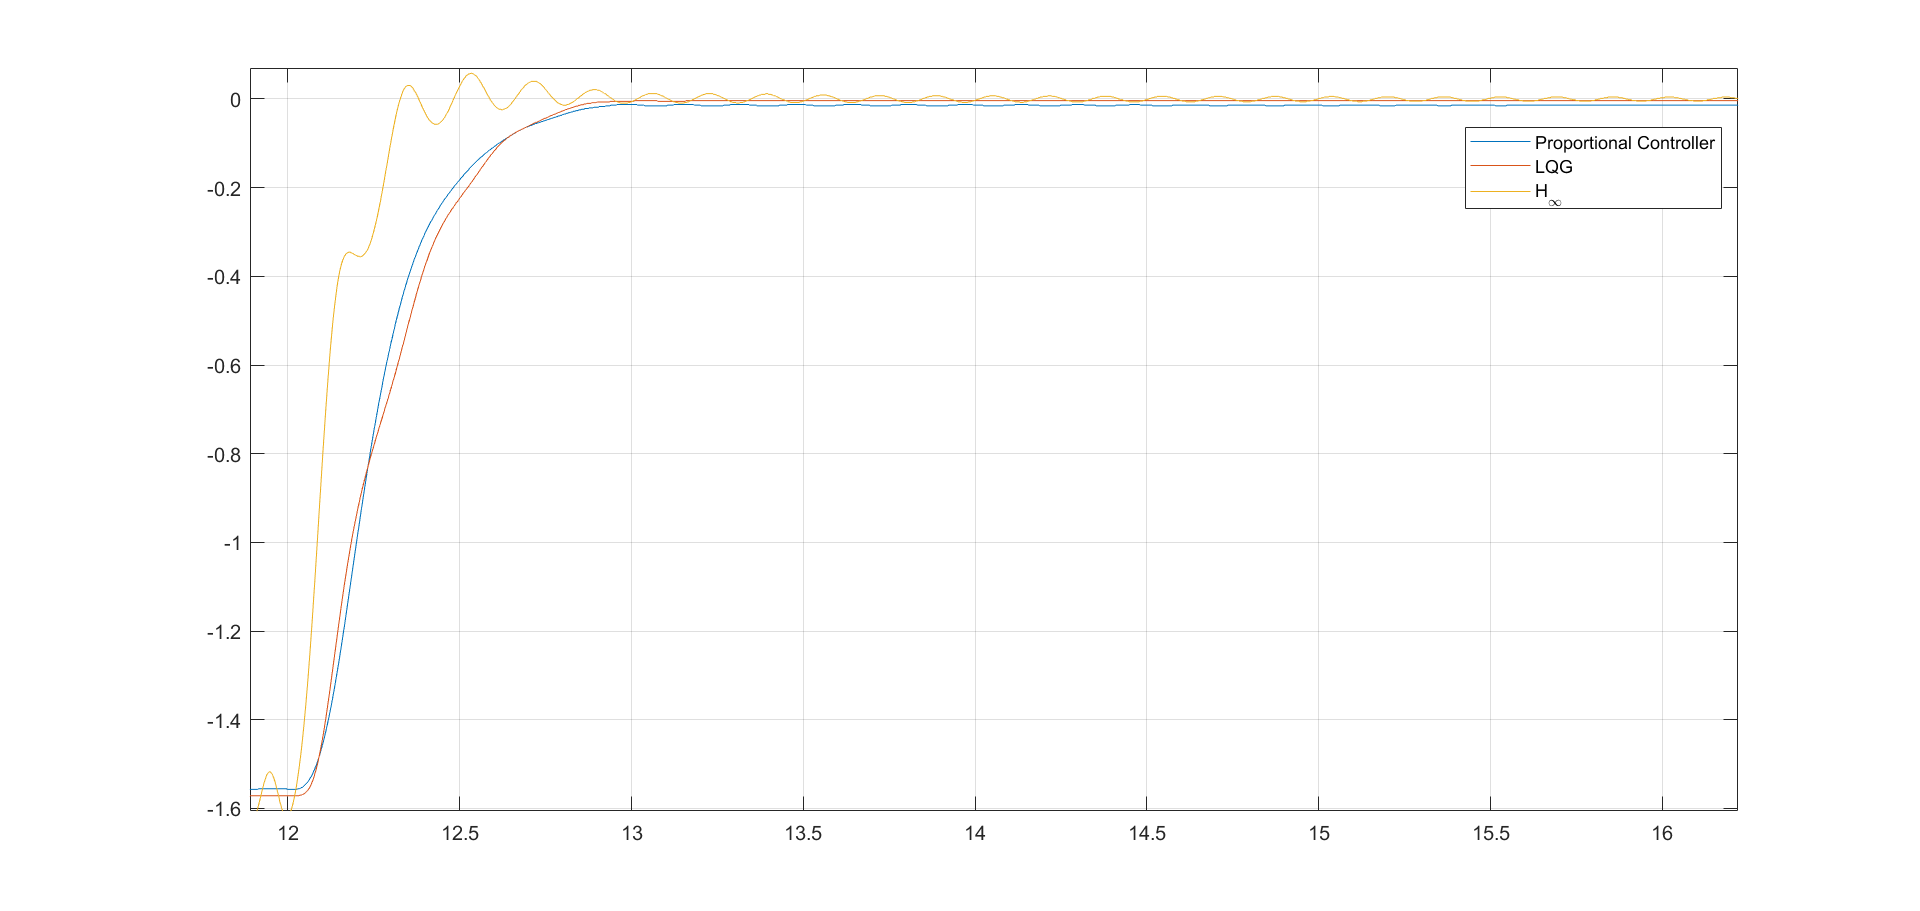
\includegraphics[width=\textwidth]{comparison_voltage_1}
	\end{subfigure}
	\begin{subfigure}{0.45\columnwidth}
		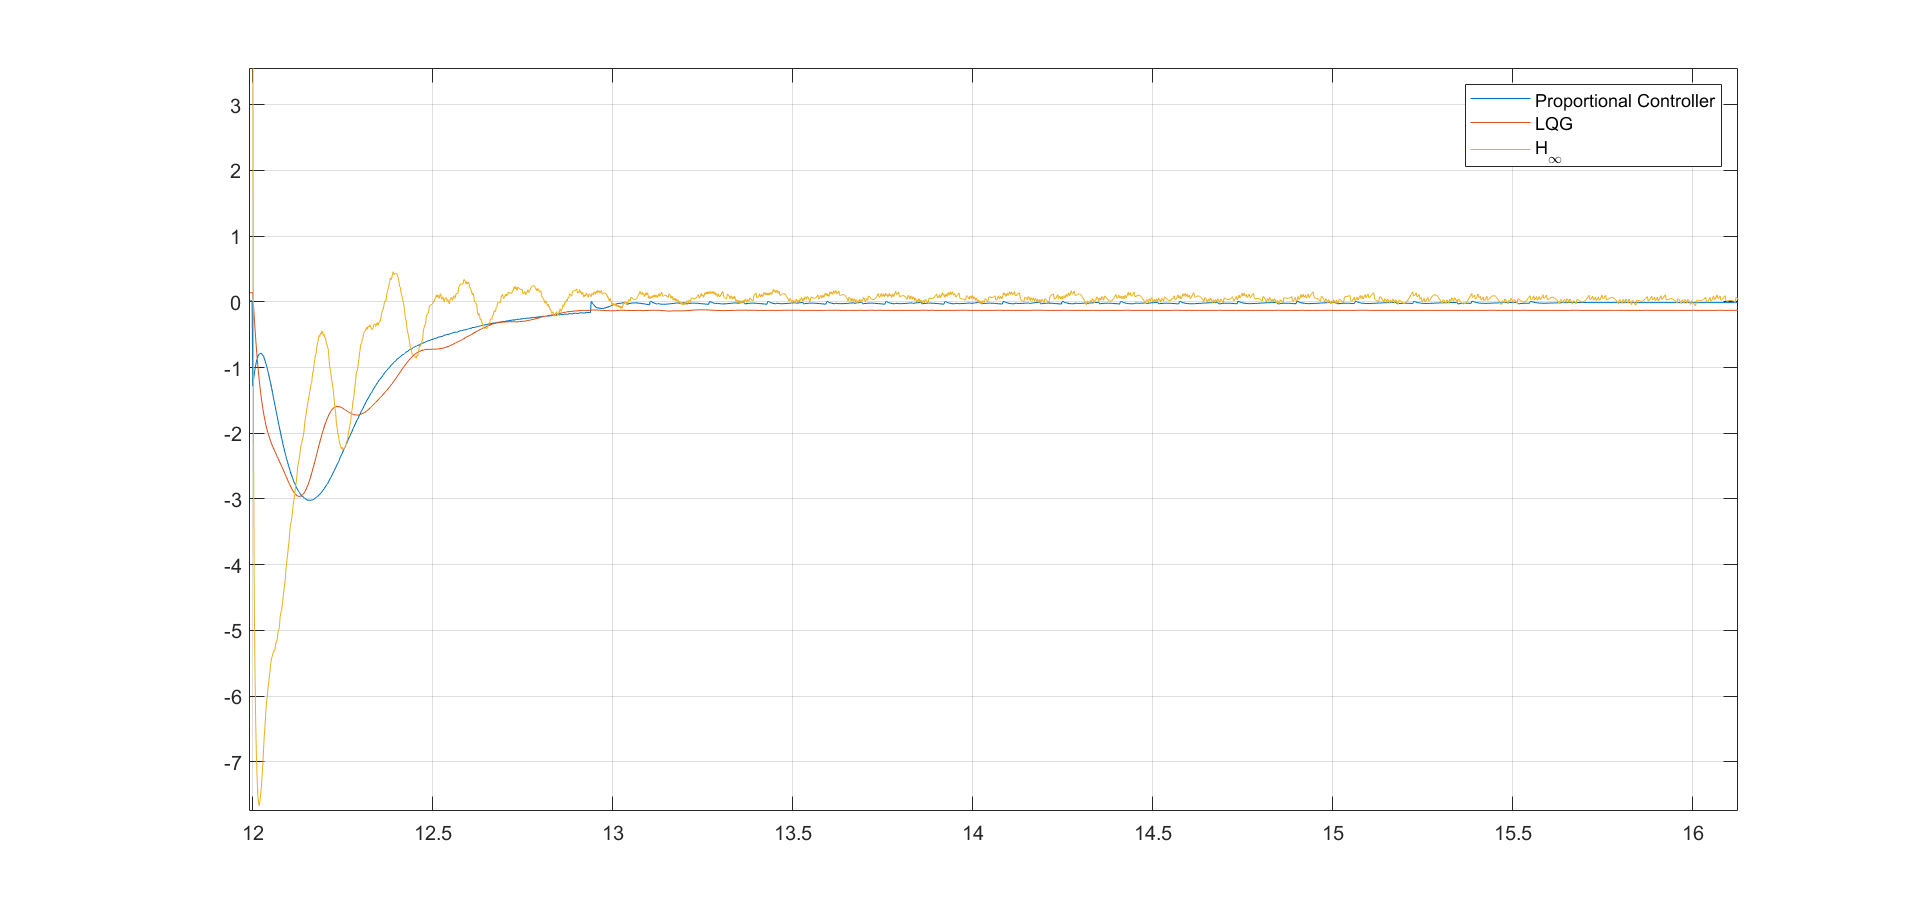
\includegraphics[width=\textwidth]{comparison_1}
	\end{subfigure}
	\caption{Different control tecnhiques for the 1 DOF case}
	\label{fig:comparison1}
\end{figure*}

\par From \cref{fig:comparison1} it is possible to notice that the $LQG$ approach and the frequency domain regulator are quite similar. The only difference arises at steady state where the $LQG$ has no oscillations. On the other hand the $H_{\infty}$ has a really different behaviour: the settling time is more than halved, but the oscillations are not negligible. For the above-mentioned reasons, the best solution is provided by the $LQG$ but nevertheless the $H_{\infty}$, if improved, might lead to an even better result.
\par
As regards the 2-DOF case, the situation is different. $LQG$ solution brings about a significant improvement with respect to the frequency domain regulator, both on settling time and oscillations point of view. Furthermore also the $H_{\infty}$ is enhanced and it can be used whenever a really fast controller is required, but on the other hand, some oscillation should be accepted. Instead, if there are not these kind of constrains and a smoother solution is prefered, it is advisable to implement the $LQG$ approach.

\begin{figure*}[h]
	\centering
	\begin{subfigure}{0.45\columnwidth}
		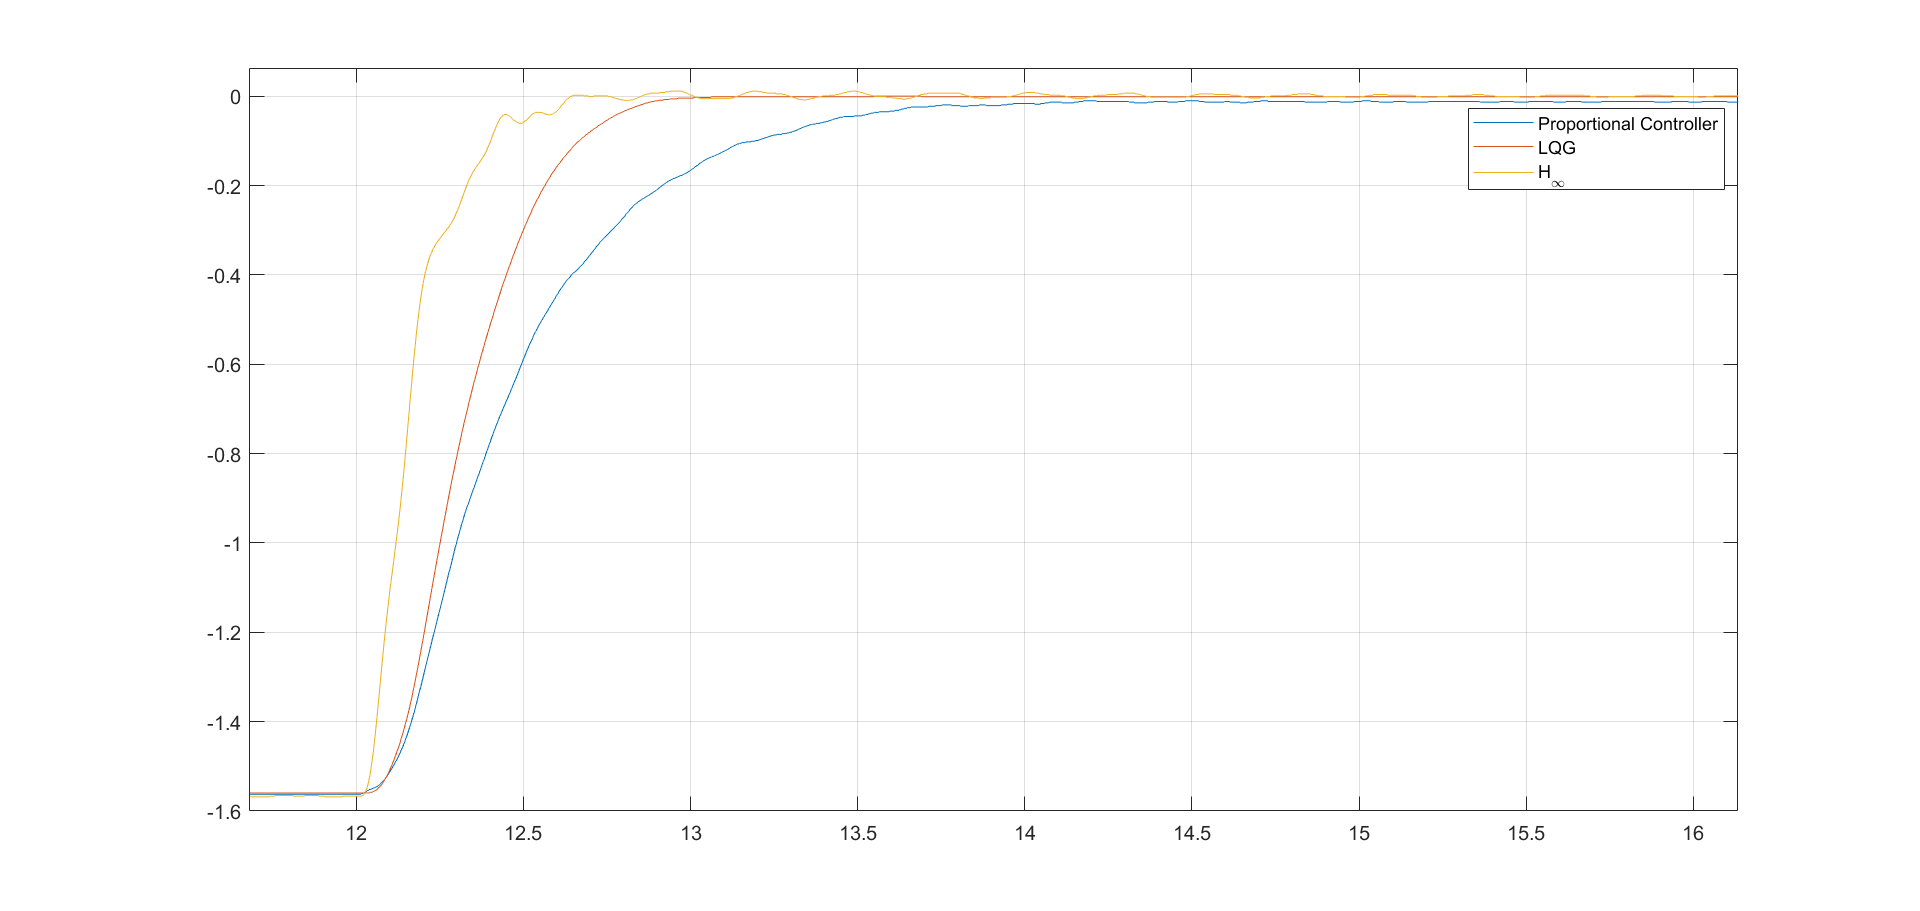
\includegraphics[width=\textwidth]{comparison_2}
	\end{subfigure}
	\begin{subfigure}{0.45\columnwidth}
		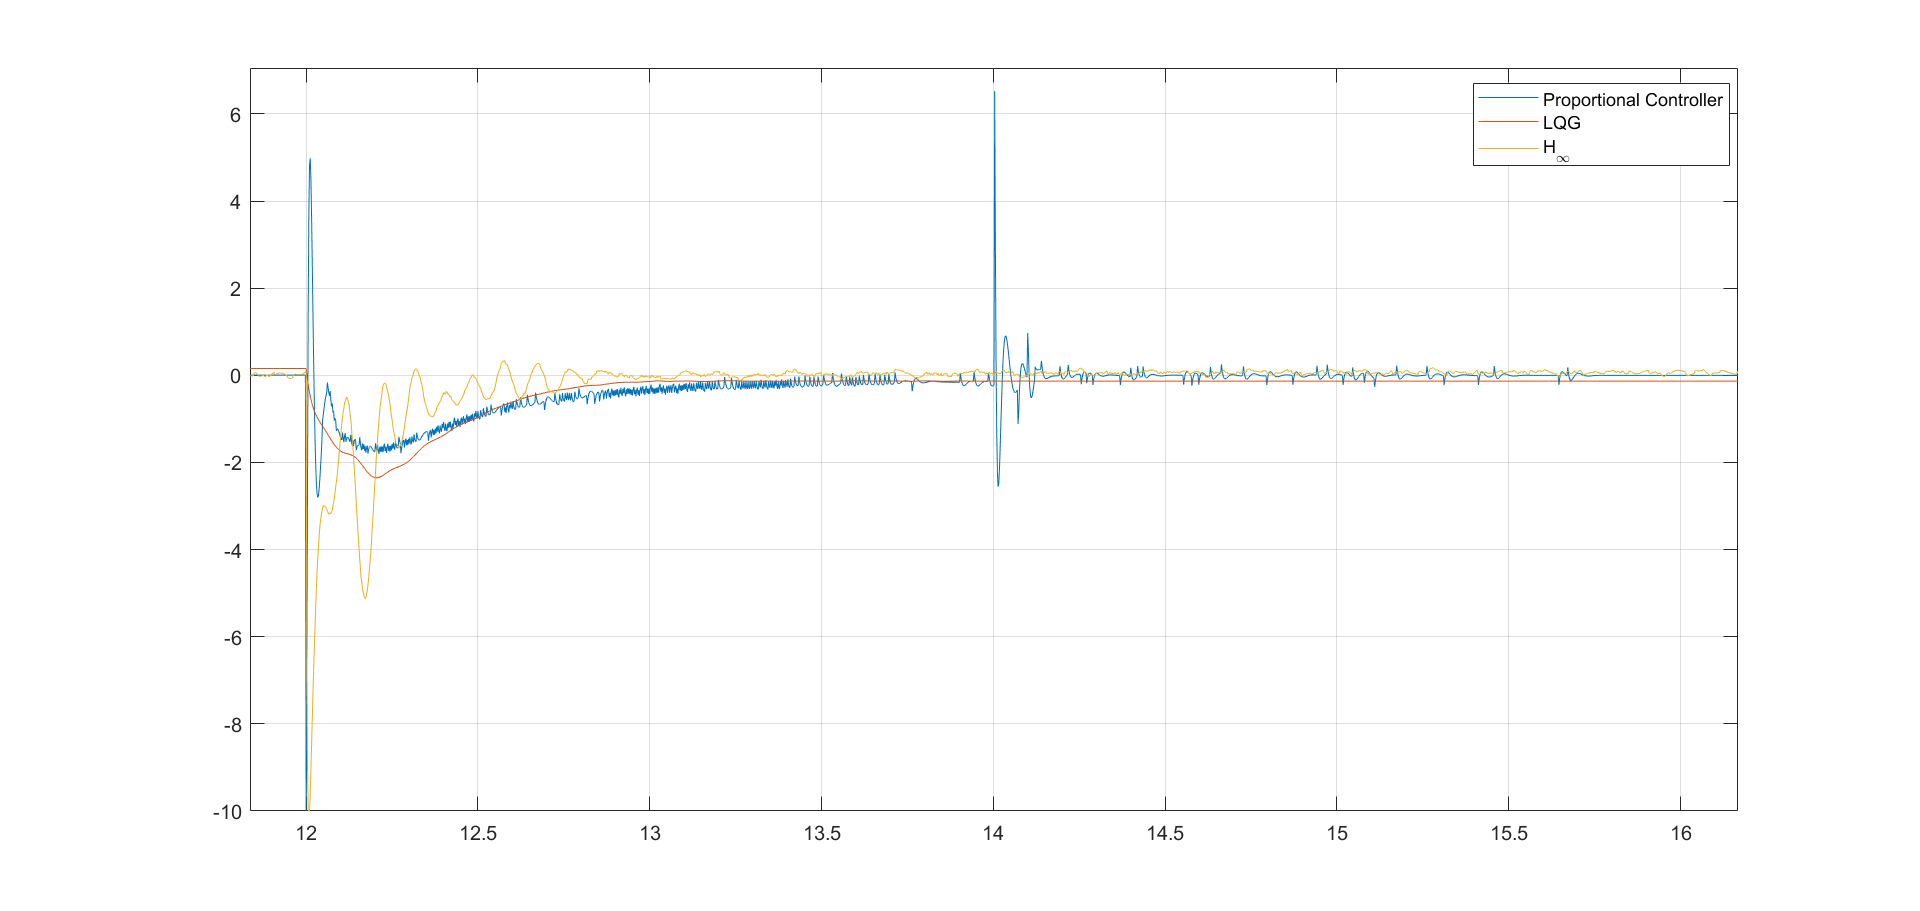
\includegraphics[width=\textwidth]{comparison_voltage_2}
	\end{subfigure}
	\caption{Different control tecnhiques for the 2 DOF case}
	\label{fig:comparison1}
\end{figure*}
\par
To conclude, most of the issues faced during the project were caused by some identification uncertainties of dominant poles or resonance peaks.
A signficant improvement would be obtained by substituting the potentiometer with an encoder, making so the motor position measurement more reliable.